\documentclass{beamer}
\usepackage[utf8]{inputenc}

\usepackage{utopia} %font utopia imported

\usetheme{Madrid}
\usecolortheme{default}

%------------------------------------------------------------
%This block of code defines the information to appear in the
%Title page
\title[Deep Variant] %optional
{Deep Variant implementation and algorithms}

\subtitle{A short story}

\author[Raimundo] % (optional)
{F. Raimundo\inst{1}}

\institute[] % (optional)
{
  \inst{1}%
  CEDAR\\
  École Polytechnique
}

\date[] % (optional)
{21th September 2017}

%\logo{\includegraphics[height=1.5cm]{lion-logo.png}}

%End of title page configuration block
%------------------------------------------------------------



%------------------------------------------------------------
%The next block of commands puts the table of contents at the 
%beginning of each section and highlights the current section:

\AtBeginSection[]
{
  \begin{frame}
    \frametitle{Table of Contents}
    \tableofcontents[currentsection]
  \end{frame}
}
%------------------------------------------------------------


\begin{document}

%The next statement creates the title page.
\frame{\titlepage}

\begin{frame}
\frametitle{DeepVariant Paper}

\begin{block}{Original Paper}
"Creating a universal SNP and small indel variant caller with deep neural networks"\\
Ryan Poplin, Dan Newburger, Jojo Dijamco, Nam Nguyen, Dion Loy, Sam Gross, Cory Y. McLean,
Mark A. DePristo\\
DOI: https://doi.org/10.1101/092890
\end{block}

\end{frame}

%---------------------------------------------------------
%This block of code is for the table of contents after
%the title page
\begin{frame}
\frametitle{Table of Contents}
\tableofcontents
\end{frame}
%---------------------------------------------------------

\section{Motivation}

\begin{frame}
    \frametitle{FDA precision challenge}

    Objectives
    \begin{itemize}
        \item Created with the Genome in a Bottle Consortium.
        \item Only one dataset with high quality annotations available (NA12878).
        \item Quality tested on new datasets.
        \item Evaluation of FScore, recall and precision for SNPs and Indels.
    \end{itemize}

\end{frame}

\begin{frame}
    \frametitle{Deep Variant results}

    \begin{itemize}
        \item Best FScore for SNPs, honorable mention for precision and recall.
        \item First method to use Deep Learning (DL).
        \item Proof of concept that DL is a promising method.
    \end{itemize}
\end{frame}

\section{Preprocessing}

%---------------------------------------------------------
%Changing visivility of the text
\begin{frame}
    \frametitle{Haplotype-aware realignment of reads}

    \begin{itemize}
        \item Reads are previously mapped (method unspecified).
        \item Candidates windows (size unspecified) are chosen based on mismatches and soft clips.
        \item Creation of De-Bruijn graphs for kmers of size 20 to 75 (increment of 5) for the
              reference and all overlapping reads in the window.
        \item Edges are weighted according to their number of occurences.
    \end{itemize}
\end{frame}

\begin{frame}
    \frametitle{Haplotype-aware realignment of reads (cont)}

    \begin{itemize}
        \item Edges with weight ower than 3 are trimmed (except for reference).
        \item Candidates haplotype are selected by traversing the graph, the two most likel are
              selected (evaluated with HMM).
        \item Reads are realigned with Smith-Waterson with affine gap penality.
        \item Position and CIGAR strings are updated in the reads.
    \end{itemize}
\end{frame}

\begin{frame}
    \frametitle{Finding candidate variants}

    \begin{itemize}
        \item Each position in the genome is evaluated.
        \item Collect all reads overlaping that position and aligned.
        \item Each possible allele is considered.
        \item If it is not reference, is present at least a number of time and represents a certain
            fraction of alleles it is emitted as a candidate.
    \end{itemize}

\end{frame}

\begin{frame}
    \frametitle{Comparative with GATK}

    \begin{itemize}
        \item No VQSR.
        \item No first pass of HaplotypeCaller.
        \item Mark duplicates used, but not described.
    \end{itemize}

\end{frame}

\begin{frame}
    \frametitle{Prepocessing conclusion}

    \begin{itemize}
        \item The realignment can be skipped (with lower results, only done for not illumina).
        \item The candidates are emitted with high sensitivity and low specificity on purpose.
        \item This whole step can be skipped (by using provided candidates).
    \end{itemize}

\end{frame}

\section{Transformation to image}

%---------------------------------------------------------
%Highlighting text
\begin{frame}
    \frametitle{Property of the image}

    \begin{itemize}
        \item An 221x100px image is created for each candidate variant.
        \item First 5 rows are for the reference genome.
        \item Each row below is used for an overlapping read.
        \item Each column encodes for the base pair at that position (relative to the ref) in the
            row of the read.
        \item Reads are thus 221bp long and there is at most 95 reads.
        \item Center column is assumed (by me) to be the position of the candidate.
    \end{itemize}

\end{frame}

\begin{frame}
    \frametitle{Pixel encoding}

    \begin{itemize}
        \item Red: encodes the base color (A: 250, G: 180, T: 100, C: 30)
        \item Green: encodes the quality (intensity linear in the quality). 
        \item Blue: direction of the strand (70 if positive, 240 otherwise).
        \item Alpha: encodes if the read is equal to the ref and if there is an alternative allele.
    \end{itemize}

\end{frame}
%---------------------------------------------------------

\section{Classifier: Training and Evaluation}

\begin{frame}
    \frametitle{Overview}
    \begin{figure}
        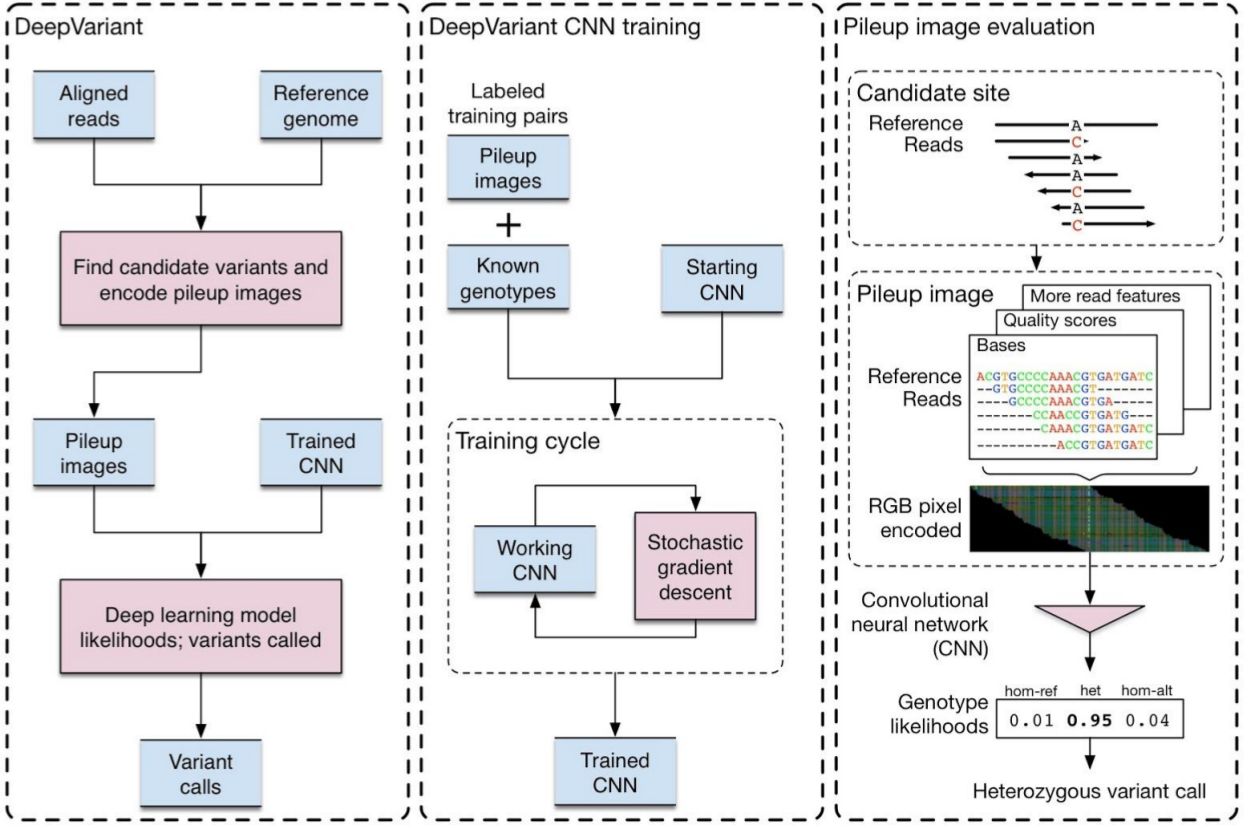
\includegraphics[width=0.8\textwidth]{deep_variant_image.png}
        \caption{DeepVariant overview}
    \end{figure}
\end{frame}

\begin{frame}
    \frametitle{Problem statement}

    \begin{itemize}
        \item Supervised.
        \item Classification into "hom-ref", "het", "hom-alt".
        \item Ground truth comes from NA12878.
        \item Trained on chr1-18, hyperparam tuned on chr19, test on chr20-22.
    \end{itemize}
\end{frame}

\begin{frame}
    \frametitle{Neural architecture}

    \begin{itemize}
        \item Inception v2.
        \item Pretrained on ImageNet.
        \item Used DistBelief framework (to be replaced with TensorFlow).
    \end{itemize}
\end{frame}

\begin{frame}
    \frametitle{Training}

    \begin{itemize}
        \item 9 partitions.
        \item Last layer initialised with gaussian random weights.
        \item SGD with 32 images per batch and 8 replicates.
        \item Training stoped after 80 hours or 250.000 epochs or training accuracy convergence.
    \end{itemize}
\end{frame}

\begin{frame}
    \frametitle{Evaluation against GATK}

    \begin{itemize}
        \item GATK implemented following Best practices and VQSR for all chr.
        \item GATK implemented following Best practices and VQSR for chr1-18.
        \item Beats both.
    \end{itemize}
\end{frame}

\begin{frame}
    \frametitle{Evaluation on Mice}

    \begin{itemize}
        \item Used MGP data.
        \item Beats state of the art (F1: 98.29\% vs 97.84\%).
        \item Gets better results when trained on NA12878 than mouse genome.
        \item Implies transfer learning accross species.
    \end{itemize}
\end{frame}

\begin{frame}
    \frametitle{Evaluation on other sequencers}

    Consistently beats other methods on
    \begin{itemize}
        \item Ion AmpliSeq exome
        \item Illumina TruSeq Genome
        \item 10x Chromium 75x WGS
        \item PacBio raw reads 40x WGS
        \item SOLID 85x
    \end{itemize}
\end{frame}

\begin{frame}
    \frametitle{Evaluation on other sequencers (cont)}

    \begin{itemize}
        \item Used realigned data from GiaB (local realignment was tuned for Illumina WGS).
        \item Retrained the CNN on the data from the new sequencers.
        \item Sugests that DeepVariant can learn on all sequencers.
        \item Sugests that DeepVariant is not too sensible to realignment method.
    \end{itemize}
\end{frame}

\section{Promises of DeepVariant}

\begin{frame}
    \frametitle{Proof of concept for Deep Learning}

    \begin{itemize}
        \item DeepVariant got best Fscore on FDA truth challenge.
        \item Only team to use Deep Learning and beat state of the Art.
        \item Suggests Deep Learning is an appropriate tool.
        \item Model had no prior on genomic data and representation was suboptimal.
    \end{itemize}
\end{frame}

\begin{frame}
    \frametitle{Opportunities}

    \begin{itemize}
        \item Transfer accross species opens the door for a unique caller for all species trained on
            all species.
        \item Retraining on different sequencing means that expert parameter tuning for each
            sequencer might be a thing of the past.
        \item Success in small variant calling migth be pushed to structural variants where state of
            the art is more art than science.
    \end{itemize}
\end{frame}

\begin{frame}
    \frametitle{Population genomics}

    \begin{itemize}
        \item Training a model on multiple samples teaches priors, which are the definition of
            population genomics.
        \item Model can be trained online with new incoming data, promising better performances as
            time goes on.
    \end{itemize}
\end{frame}

\begin{frame}
    \frametitle{Latency}

    \begin{itemize}
        \item Computation cost of the trained model are only dependent on the size of the image
            (here 299x299px).
        \item Deep Learning training methods are easily distributed (see DistBelief).
        \item Main bottleneck are preprocessing and image creation (assumed).
        \item Smaller models can be learned (see Distill).
    \end{itemize}
\end{frame}

\end{document}
